\tikzset{every picture/.style={line width=0.75pt}} %set default line width to 0.75pt

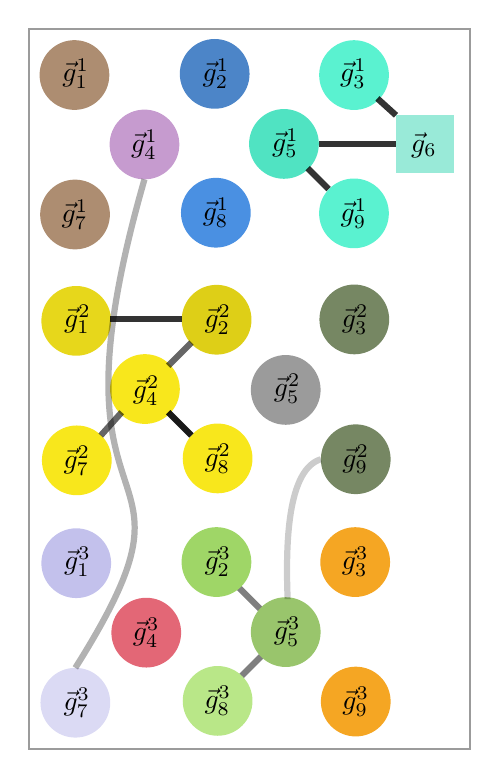
\begin{tikzpicture}[x=0.75pt,y=0.75pt,yscale=-0.56,xscale=0.56]
%uncomment if require: \path (0,1438); %set diagram left start at 0, and has height of 1438

%Shape: Rectangle [id:dp5381136388503212]
\draw  [color={rgb, 255:red, 155; green, 155; blue, 155 }  ,draw opacity=1 ] (20,700) -- (20,80) -- (400,80) -- (400,700) -- cycle ;

%Shape: Rectangle [id:dp39137146349868646]
%\draw  [color={rgb, 255:red, 155; green, 155; blue, 155 }  ,draw opacity=1 ] (21.53,491.52) -- (20.73,291.53) -- (400.72,290) -- (401.53,490) -- cycle ;

%Shape: Rectangle [id:dp3461506815581068]
%\draw  [color={rgb, 255:red, 155; green, 155; blue, 155 }  ,draw opacity=1 ] (21.53,700) -- (20.73,500) -- (400.72,498.48) -- (401.53,698.47) -- cycle ;


%Shape: Circle [id:dp12286992130015428]
\draw  [draw opacity=0][fill={rgb, 255:red, 173; green, 141; blue, 113 }  ,fill opacity=1 ] (29.84,239.84) .. controls (29.84,223.27) and (43.27,209.84) .. (59.84,209.84) .. controls (76.41,209.84) and (89.84,223.27) .. (89.84,239.84) .. controls (89.84,256.41) and (76.41,269.84) .. (59.84,269.84) .. controls (43.27,269.84) and (29.84,256.41) .. (29.84,239.84) -- cycle ;
%Shape: Circle [id:dp7931751449222735]
\draw  [draw opacity=0][fill={rgb, 255:red, 173; green, 141; blue, 113 }  ,fill opacity=1 ] (29.36,119.84) .. controls (29.36,103.27) and (42.79,89.84) .. (59.36,89.84) .. controls (75.93,89.84) and (89.36,103.27) .. (89.36,119.84) .. controls (89.36,136.41) and (75.93,149.84) .. (59.36,149.84) .. controls (42.79,149.84) and (29.36,136.41) .. (29.36,119.84) -- cycle ;
%Shape: Circle [id:dp16673433726568354]
\draw  [draw opacity=0][fill={rgb, 255:red, 170; green, 106; blue, 183 }  ,fill opacity=0.67 ] (89.6,179.6) .. controls (89.6,163.03) and (103.03,149.6) .. (119.6,149.6) .. controls (136.17,149.6) and (149.6,163.03) .. (149.6,179.6) .. controls (149.6,196.17) and (136.17,209.6) .. (119.6,209.6) .. controls (103.03,209.6) and (89.6,196.17) .. (89.6,179.6) -- cycle ;
%Shape: Circle [id:dp15511724636448365]
\draw  [draw opacity=0][fill={rgb, 255:red, 74; green, 144; blue, 226 }  ,fill opacity=1 ] (151,238.31) .. controls (151,221.74) and (164.43,208.31) .. (181,208.31) .. controls (197.57,208.31) and (211,221.74) .. (211,238.31) .. controls (211,254.88) and (197.57,268.31) .. (181,268.31) .. controls (164.43,268.31) and (151,254.88) .. (151,238.31) -- cycle ;
%Shape: Circle [id:dp8495812213022542]
\draw  [draw opacity=0][fill={rgb, 255:red, 76; green, 133; blue, 200 }  ,fill opacity=1 ] (150,118.85) .. controls (150,102.28) and (163.44,88.85) .. (180,88.85) .. controls (196.57,88.85) and (210,102.28) .. (210,118.85) .. controls (210,135.42) and (196.57,148.85) .. (180,148.85) .. controls (163.44,148.85) and (150,135.42) .. (150,118.85) -- cycle ;
%Shape: Circle [id:dp46577960716750777]
\draw  [draw opacity=0][fill={rgb, 255:red, 80; green, 227; blue, 194 }  ,fill opacity=1 ] (209.6,179.12) .. controls (209.6,162.55) and (223.03,149.12) .. (239.6,149.12) .. controls (256.17,149.12) and (269.6,162.55) .. (269.6,179.12) .. controls (269.6,195.69) and (256.17,209.12) .. (239.6,209.12) .. controls (223.03,209.12) and (209.6,195.69) .. (209.6,179.12) -- cycle ;
%Shape: Circle [id:dp30991147509029027]
\draw  [draw opacity=0][fill={rgb, 255:red, 90; green, 242; blue, 208 }  ,fill opacity=1 ] (269.84,238.88) .. controls (269.84,222.31) and (283.27,208.88) .. (299.84,208.88) .. controls (316.41,208.88) and (329.84,222.31) .. (329.84,238.88) .. controls (329.84,255.44) and (316.41,268.88) .. (299.84,268.88) .. controls (283.27,268.88) and (269.84,255.44) .. (269.84,238.88) -- cycle ;
%Shape: Circle [id:dp10962416440320566]
\draw  [draw opacity=0][fill={rgb, 255:red, 90; green, 242; blue, 208 }  ,fill opacity=1 ] (269.88,119.88) .. controls (269.88,103.31) and (283.31,89.88) .. (299.88,89.88) .. controls (316.45,89.88) and (329.88,103.31) .. (329.88,119.88) .. controls (329.88,136.45) and (316.45,149.88) .. (299.88,149.88) .. controls (283.31,149.88) and (269.88,136.45) .. (269.88,119.88) -- cycle ;

%Shape: Circle [id:dp13607314793635106]
\draw  [draw opacity=0][fill={rgb, 255:red, 248; green, 231; blue, 28 }  ,fill opacity=1 ] (31.37,451.36) .. controls (31.37,434.8) and (44.8,421.36) .. (61.37,421.36) .. controls (77.94,421.36) and (91.37,434.8) .. (91.37,451.36) .. controls (91.37,467.93) and (77.94,481.36) .. (61.37,481.36) .. controls (44.8,481.36) and (31.37,467.93) .. (31.37,451.36) -- cycle ;
%Shape: Circle [id:dp22834187586321186]
\draw  [draw opacity=0][fill={rgb, 255:red, 231; green, 215; blue, 27 }  ,fill opacity=1 ] (30.89,331.36) .. controls (30.89,314.8) and (44.32,301.36) .. (60.89,301.36) .. controls (77.46,301.36) and (90.89,314.8) .. (90.89,331.36) .. controls (90.89,347.93) and (77.46,361.36) .. (60.89,361.36) .. controls (44.32,361.36) and (30.89,347.93) .. (30.89,331.36) -- cycle ;
%Shape: Circle [id:dp9030431506925378]
\draw  [draw opacity=0][fill={rgb, 255:red, 248; green, 231; blue, 28 }  ,fill opacity=1 ] (90,390) .. controls (90,373.43) and (103.43,360) .. (120,360) .. controls (136.57,360) and (150,373.43) .. (150,390) .. controls (150,406.57) and (136.57,420) .. (120,420) .. controls (103.43,420) and (90,406.57) .. (90,390) -- cycle ;
%Shape: Circle [id:dp5036111314358263]
\draw  [draw opacity=0][fill={rgb, 255:red, 248; green, 231; blue, 28 }  ,fill opacity=1 ] (152.52,449.71) .. controls (152.52,433.15) and (165.96,419.71) .. (182.52,419.71) .. controls (199.09,419.71) and (212.52,433.15) .. (212.52,449.71) .. controls (212.52,466.28) and (199.09,479.71) .. (182.52,479.71) .. controls (165.96,479.71) and (152.52,466.28) .. (152.52,449.71) -- cycle ;
%Shape: Circle [id:dp28094865389913615]
\draw  [draw opacity=0][fill={rgb, 255:red, 222; green, 207; blue, 23 }  ,fill opacity=1 ] (151.65,330.38) .. controls (151.65,313.81) and (165.08,300.38) .. (181.65,300.38) .. controls (198.22,300.38) and (211.65,313.81) .. (211.65,330.38) .. controls (211.65,346.94) and (198.22,360.38) .. (181.65,360.38) .. controls (165.08,360.38) and (151.65,346.94) .. (151.65,330.38) -- cycle ;
%Shape: Circle [id:dp8199553596351965]
\draw  [draw opacity=0][fill={rgb, 255:red, 155; green, 155; blue, 155 }  ,fill opacity=1 ] (211.13,390.76) .. controls (211.13,374.19) and (224.56,360.76) .. (241.13,360.76) .. controls (257.7,360.76) and (271.13,374.19) .. (271.13,390.76) .. controls (271.13,407.33) and (257.7,420.76) .. (241.13,420.76) .. controls (224.56,420.76) and (211.13,407.33) .. (211.13,390.76) -- cycle ;
%Shape: Circle [id:dp061627101972308695]
\draw  [draw opacity=0][fill={rgb, 255:red, 34; green, 61; blue, 3 }  ,fill opacity=0.62 ] (271.37,450.4) .. controls (271.37,433.83) and (284.8,420.4) .. (301.37,420.4) .. controls (317.94,420.4) and (331.37,433.83) .. (331.37,450.4) .. controls (331.37,466.97) and (317.94,480.4) .. (301.37,480.4) .. controls (284.8,480.4) and (271.37,466.97) .. (271.37,450.4) -- cycle ;
%Shape: Circle [id:dp6586711959399798]
\draw  [draw opacity=0][fill={rgb, 255:red, 34; green, 61; blue, 3 }  ,fill opacity=0.62 ] (270.12,330.12) .. controls (270.12,313.55) and (283.55,300.12) .. (300.12,300.12) .. controls (316.69,300.12) and (330.12,313.55) .. (330.12,330.12) .. controls (330.12,346.69) and (316.69,360.12) .. (300.12,360.12) .. controls (283.55,360.12) and (270.12,346.69) .. (270.12,330.12) -- cycle ;
%Straight Lines [id:da09795376579003179]
\draw [color={rgb, 255:red, 0; green, 0; blue, 0 }  ,draw opacity=0.5 ][line width=2.25]    (200,640) -- (220,620) ;
%Straight Lines [id:da13253659772522353]
\draw [color={rgb, 255:red, 0; green, 0; blue, 0 }  ,draw opacity=0.5 ][line width=2.25]    (200,560) -- (220,580) ;

%Shape: Circle [id:dp07594340015479584]
\draw  [draw opacity=0][fill={rgb, 255:red, 195; green, 193; blue, 236 }  ,fill opacity=0.6 ] (30.12,659.88) .. controls (30.12,643.31) and (43.55,629.88) .. (60.12,629.88) .. controls (76.69,629.88) and (90.12,643.31) .. (90.12,659.88) .. controls (90.12,676.45) and (76.69,689.88) .. (60.12,689.88) .. controls (43.55,689.88) and (30.12,676.45) .. (30.12,659.88) -- cycle ;
%Shape: Circle [id:dp6610712869287463]
\draw  [draw opacity=0][fill={rgb, 255:red, 195; green, 193; blue, 236 }  ,fill opacity=1 ] (30.89,539.84) .. controls (30.89,523.27) and (44.32,509.84) .. (60.89,509.84) .. controls (77.46,509.84) and (90.89,523.27) .. (90.89,539.84) .. controls (90.89,556.41) and (77.46,569.84) .. (60.89,569.84) .. controls (44.32,569.84) and (30.89,556.41) .. (30.89,539.84) -- cycle ;
%Shape: Circle [id:dp7622423737356947]
\draw  [draw opacity=0][fill={rgb, 255:red, 208; green, 2; blue, 27 }  ,fill opacity=0.6 ] (121.25,629.6) .. controls (104.68,629.67) and (91.19,616.29) .. (91.13,599.72) .. controls (91.06,583.15) and (104.44,569.67) .. (121.01,569.6) .. controls (137.58,569.53) and (151.06,582.91) .. (151.13,599.48) .. controls (151.19,616.05) and (137.82,629.53) .. (121.25,629.6) -- cycle ;
%Shape: Circle [id:dp4084876787586895]
\draw  [draw opacity=0][fill={rgb, 255:red, 185; green, 231; blue, 136 }  ,fill opacity=1 ] (152.52,658.31) .. controls (152.52,641.74) and (165.96,628.31) .. (182.52,628.31) .. controls (199.09,628.31) and (212.52,641.74) .. (212.52,658.31) .. controls (212.52,674.88) and (199.09,688.31) .. (182.52,688.31) .. controls (165.96,688.31) and (152.52,674.88) .. (152.52,658.31) -- cycle ;
%Shape: Circle [id:dp5875693847671164]
\draw  [draw opacity=0][fill={rgb, 255:red, 159; green, 214; blue, 103 }  ,fill opacity=1 ] (151.53,538.85) .. controls (151.53,522.28) and (164.96,508.85) .. (181.53,508.85) .. controls (198.1,508.85) and (211.53,522.28) .. (211.53,538.85) .. controls (211.53,555.42) and (198.1,568.85) .. (181.53,568.85) .. controls (164.96,568.85) and (151.53,555.42) .. (151.53,538.85) -- cycle ;
%Shape: Circle [id:dp06003724860547344]
\draw  [draw opacity=0][fill={rgb, 255:red, 153; green, 197; blue, 108 }  ,fill opacity=1 ] (211.13,599.12) .. controls (211.13,582.55) and (224.56,569.12) .. (241.13,569.12) .. controls (257.7,569.12) and (271.13,582.55) .. (271.13,599.12) .. controls (271.13,615.69) and (257.7,629.12) .. (241.13,629.12) .. controls (224.56,629.12) and (211.13,615.69) .. (211.13,599.12) -- cycle ;
%Shape: Circle [id:dp3947958928282629]
\draw  [draw opacity=0][fill={rgb, 255:red, 245; green, 166; blue, 35 }  ,fill opacity=1 ] (271.37,658.88) .. controls (271.37,642.31) and (284.8,628.88) .. (301.37,628.88) .. controls (317.94,628.88) and (331.37,642.31) .. (331.37,658.88) .. controls (331.37,675.44) and (317.94,688.88) .. (301.37,688.88) .. controls (284.8,688.88) and (271.37,675.44) .. (271.37,658.88) -- cycle ;
%Shape: Circle [id:dp18102804016986096]
\draw  [draw opacity=0][fill={rgb, 255:red, 245; green, 166; blue, 35 }  ,fill
opacity=1 ] (270.89,538.88) .. controls (270.89,522.31) and (284.32,508.88)
.. (300.89,508.88) .. controls (317.45,508.88) and (330.89,522.31)
.. (330.89,538.88) .. controls (330.89,555.45) and (317.45,568.88)
.. (300.89,568.88) .. controls (284.32,568.88) and (270.89,555.45)
.. (270.89,538.88) -- cycle ;
%Curve Lines [id:da3377087525660538] 
\draw [color={rgb, 255:red, 0; green, 0; blue, 0 }  ,draw opacity=0.3 ][line width=2.25]    (119.6,209.6) .. controls (25.8,536) and (186.8,429) .. (60.12,629.88) ;
%Straight Lines [id:da43642919945499603]
\draw [color={rgb, 255:red, 0; green, 0; blue, 0 }  ,draw opacity=0.8 ][line width=2.25]    (90,330) -- (152,330) ; %remember!
%Straight Lines [id:da8359064659577915]
\draw [color={rgb, 255:red, 0; green, 0; blue, 0 }  ,draw opacity=0.6 ][line width=2.25]    (140,370) -- (160,350) ;
%Straight Lines [id:da367274331259694]
\draw [color={rgb, 255:red, 0; green, 0; blue, 0 }  ,draw opacity=0.6 ][line width=2.25]    (82,430) -- (100,410) ;
%Straight Lines [id:da7756630094250268]
\draw [color={rgb, 255:red, 0; green, 0; blue, 0 }  ,draw opacity=0.9 ][line width=2.25]    (140,410) -- (160,430) ;
%Straight Lines [id:da31290273671454116]
\draw [color={rgb, 255:red, 0; green, 0; blue, 0 }  ,draw opacity=0.8 ][line width=2.25]    (260,200) -- (278,218) ;
%Straight Lines [id:da8522668149365773]
\draw [color={rgb, 255:red, 0; green, 0; blue, 0 }  ,draw opacity=0.8 ][line width=2.25]    (336,154.5) -- (320,140) ;
%Straight Lines [id:da771798416536507]
\draw [color={rgb, 255:red, 0; green, 0; blue, 0 }  ,draw opacity=0.8 ][line width=2.25]    (269.6,179.12) -- (335.6,179.12) ;
%Curve Lines [id:da8781500202610568]
\draw [color={rgb, 255:red, 0; green, 0; blue, 0 }  ,draw opacity=0.2 ][line width=2.25]    (242.77,570.74) .. controls (240.51,513.97) and (244.58,458.67) .. (271.37,450.4) ;
%Shape: Square [id:dp2620517183205848]
\draw  [draw opacity=0][fill={rgb, 255:red, 153; green, 234; blue, 216 }  ,fill opacity=1 ] (336,154.5) -- (385.5,154.5) -- (385.5,204) -- (336,204) -- cycle ;

% Text Node
\draw (299.36,118.88) node   [align=left] {$\vec g_{3}^1$};
% Text Node
\draw (59.84,239.84) node   [align=left] {$\vec g_{7}^1$};
% Text Node
\draw (240.89,178.54) node   [align=left] {$\vec g_{5}^1$};
% Text Node
\draw (181.19,238.46) node   [align=left] {$\vec g_{8}^1$};
% Text Node
\draw (119.6,179.6) node   [align=left] {$\vec g_{4}^1$};
% Text Node
\draw (181.17,118.51) node   [align=left] {$\vec g_{2}^1$};
% Text Node
\draw (60.36,118.42) node   [align=left] {$\vec g_{1}^1$};
% Text Node
\draw (299.84,238.88) node   [align=left] {$\vec g_{9}^1$};

% Text Node
\draw (300.89,330.4) node   [align=left] {$\vec g_{3}^2$};
% Text Node
\draw (61.37,451.36) node   [align=left] {$\vec g_{7}^2$};
% Text Node
\draw (242.41,390.07) node   [align=left] {$\vec g_{5}^2$};
% Text Node
\draw (182.72,449.98) node   [align=left] {$\vec g_{8}^2$};
% Text Node
\draw (121.13,391.12) node   [align=left] {$\vec g_{4}^2$};
% Text Node
\draw (182.69,330.04) node   [align=left] {$\vec g_{2}^2$};
% Text Node
\draw (61.89,329.94) node  [align=left] {$\vec g_{1}^2$};
% Text Node
\draw (301.37,450.4) node   [align=left] {$\vec g_{9}^2$};

% Text Node
\draw (300.89,538.88) node   [align=left] {$\vec g_{3}^3$};
% Text Node
\draw (61.37,659.84) node   [align=left] {$\vec g_{7}^3$};
% Text Node
\draw (242.41,598.54) node   [align=left] {$\vec g_{5}^3$};
% Text Node
\draw (182.72,658.46) node   [align=left] {$\vec g_{8}^3$};
% Text Node
\draw (121.13,599.6) node   [align=left] {$\vec g_{4}^3$};
% Text Node
\draw (182.69,538.51) node   [align=left] {$\vec g_{2}^3$};
% Text Node
\draw (61.89,538.42) node [align=left] {$\vec g_{1}^3$};
% Text Node
\draw (301.37,658.88) node   [align=left] {$\vec g_{9}^3$};

% Text Node
\draw (360,180) node   [align=left] {$\vec g_{6}$};


\end{tikzpicture}
